\section{Gerador}

O \texttt{Generator} tem, como função, recebendo parâmetros como comprimento,
largura, raio, etc., gerar ficheiros de texto com a extensão \verb|.3d|, cujo conteúdo
é a informação sobre as figuras a criar. 

Nesta secção ir-se-á descrever o processo de desenvolvimento das figuras
necessárias do sistema solar. As figuras pertinentes a desenhar são a esfera
(para os planetas e sol) e um disco (para alguns planetas que os tenham, como
por exemplo Saturno). 



\subsection{Esfera}
%---------------------------------------------------------------------------------------------------------------%
\subsubsection{Análise do Problema}
Para a construção da esfera teve-se que ter em conta coordenadas esféricas
modificadas para o referencial rodado com Y para cima, Z como eixo das abcissas
e X como eixo das ordenadas, como demonstra a Equação~\ref{eq:equ2}.


\begin{equation}
    \begin{cases}
    x = \cos(\phi) * \sin(\theta) * \rho \\
    y = \sin(\phi) * \rho \\
    z = \cos(\phi) * \cos(\theta) *\rho
    \end{cases}
\label{eq:equ2}
\end{equation}

Na Equação~\ref{eq:equ2}, $\rho$ representa o raio, $\phi$ o ângulo polar sendo
$\phi \in [-\dfrac{\pi}{2}, \dfrac{\pi}{2}]$, $\theta$ representa o ângulo
azimutal sendo $\theta \in [0, 2\pi]$. 


\newpage
\subsubsection{Diagrama}


\begin{center}
 	
 	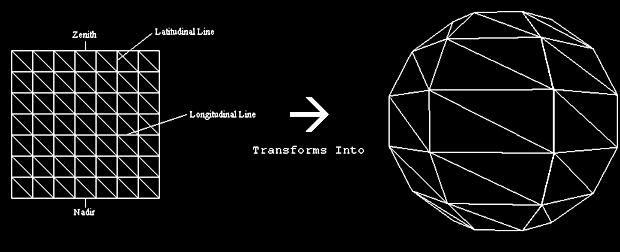
\includegraphics[width=\textwidth,height=\textheight,keepaspectratio]{resources/sphere05.jpg}
 	\captionsetup{type=figure, width=0.8\linewidth}
	\caption{Objetivo do algoritmo de construção de esfera}
\label{fig:ssec1:diagram:plane:to:sphere} 
\end{center}



\begin{center}
 	
 	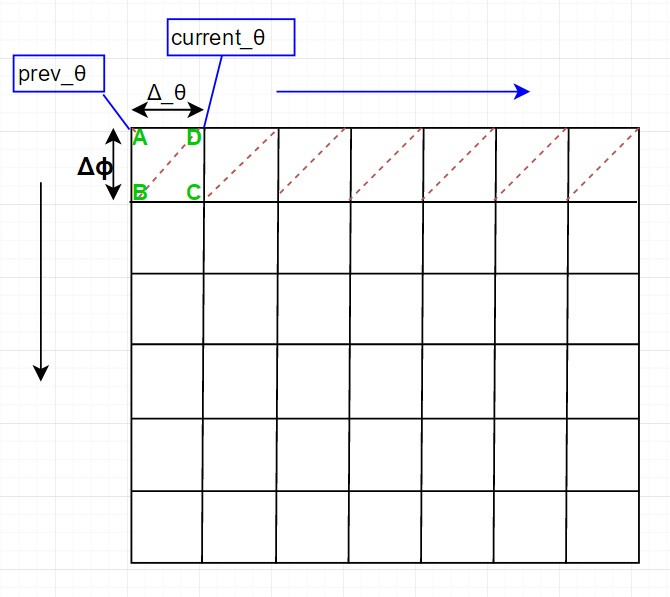
\includegraphics[keepaspectratio]{resources/esferaw.jpg}
 	\captionsetup{type=figure, width=0.8\linewidth}
	\caption{Diagrama de representativo de construção de esfera}
\label{fig:ssec1:diagram:sphere} 
\end{center}


No \emph{Figura~\ref{fig:ssec1:diagram:sphere}} pode-se ver uma matriz, que
representa a esfera nos graus de $\phi$ e $\theta$ para 6 \emph{stacks}
e 7 \emph{slices}. Assim como um mapa representativo da Terra, pretende-se
mostrar os pontos se a esfera fosse aplanada (ver
\emph{Figura~\ref{fig:ssec1:diagram:plane:to:sphere}}).

Em cada quadrícula são calculados 4 pontos iniciais, com base nos cálculos
apresentados pelo fórmula anterior. Note-se que, se usou duas variáveis para
guardar o $\phi$ anterior e o $\phi$ corrente, e $\theta$ anterior  e $\theta$
corrente. Adicionalmente é calculada a diferença de graus entre \emph{slices}
e \emph{stacks}, representados por $\Delta \phi$ e $\Delta \theta$,
respetivamente. 

A intenção é calcular cada quadricula para cada linha e coluna, com auxilio das
diferenças dos ângulos e à medida que se avança em cada quadricula, guardar
o último grau calculado ($\phi$ e $\theta$) e calcular nos pontos com
o incremento nestes ângulos. Assim desloca-se para a direita na matriz, conforme
$\theta$ avança de 0 para $2\pi$ e para baixo, conforme $\phi$ avança de
$\dfrac{\pi}{2}$ para $-\dfrac{\pi}{2}$ (sentido dos ponteiros do relógio).
O \emph{Algoritmo~\ref{alg:secc1:esfera}} representa este processo
e a \emph{Figura~\ref{fig:sec1:sphere:angles}} demonstra o que se
mencionou.  


\begin{center}
 	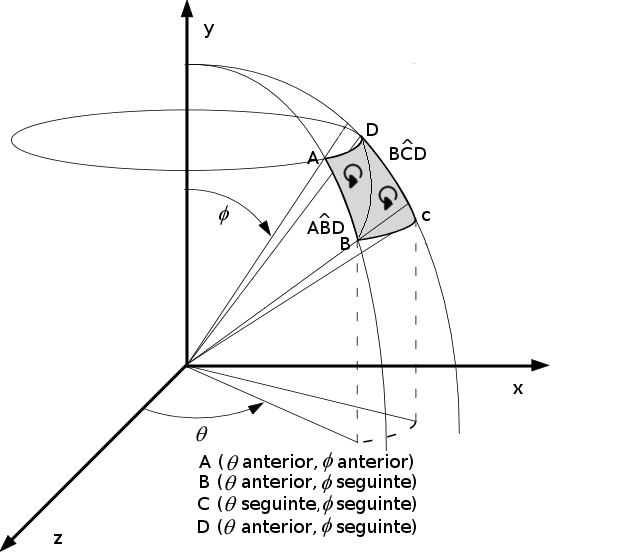
\includegraphics[width=\textwidth,height=0.5\textheight,keepaspectratio]{resources/esfera2.png}
 	\captionsetup{type=figure, width=0.8\linewidth}
	\caption{Diagrama de construção de esfera, com eixos, ordem do vértices
	e ângulos}
\label{fig:sec1:sphere:angles} 
\end{center}

O resultado pode-se ver na \emph{Figura~\ref{fig:ssec1:res:sphere}}, que
demonstra uma esfera em \emph{wireframe} gerada com a aplicação.  

\begin{center}
 	
 	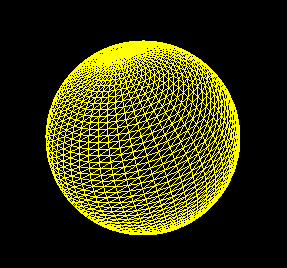
\includegraphics[keepaspectratio]{resources/sphere.png}
 	\captionsetup{type=figure, width=0.8\linewidth}
	\caption{Esfera gerada}
\label{fig:ssec1:res:sphere} 
\end{center}
\newpage

\newgeometry{margin=1cm}
\begin{landscape}
\thispagestyle{empty} %% Remove header and footer.

\begin{algorithm}
\caption{Esfera}\label{alg:secc1:esfera}

\begin{center}
%\footnotesize %% Smaller font size.

\begin{algorithmic}[1]
\State$\Delta\_\theta \gets \dfrac{2\pi}{slices}$

\State$\Delta\_\phi \gets \dfrac{2\pi}{stacks}$

\State$prev\_\phi \gets \dfrac{\pi}{2}$

\State$current\_\phi \gets prev\_\phi - \Delta\_\phi$


\State$i \gets 0$
\While{$i \leq stacks$} 


\State$prev\_\theta \gets 0$
\State$current\_\theta \gets \Delta\_\theta$

\State$j \gets 0$

\While{$j \leq slices$} 


\State$Ponto A \gets raio*\cos(prev\_\phi) * \sin(prev\_\theta)$, $
raio*\sin(prev\_\phi)$, $raio*\cos(prev\_\phi) * \cos(prev\_\theta)$
\State$Ponto B \gets raio*\cos(current\_\phi)*\sin(prev\_\theta)$,$
 raio*\sin(current\_\phi)$,$
 raio*\cos(current\_\phi) * \cos(prev\_\theta)$
\State$Ponto C \gets raio*\cos(prev\_\phi) * 
 \sin(current\_\theta),raio*\sin(prev\_\phi)$,$
 raio*\cos(prev\_\phi) * \cos(current\_\theta)$
\State$Ponto D \gets raio*\cos(current\_\phi) *
 \sin(current\_\theta)$,$raio*\sin(current\_\phi)$,$raio*\cos(current\_\phi) *  \cos(current\_\theta)$
\newline
\State$Triangulo(Ponto A, Ponto B, Ponto D)$ \Comment{Guardado em ficheiro}
\State$Triangulo(Ponto B, Ponto C, Ponto D)$ \Comment{Guardado em ficheiro}
\newline
\State$prev\_\theta \gets current\_\theta$
\State$current\_\theta \gets current\_\theta + \Delta\_\theta $
\newline
\State$j \gets j + 1$ 

\EndWhile{}

\State$prev\_\phi \gets Current\_\phi$
\State$current\_\phi \gets Current\_\phi - \Delta\_\phi $
\State$i \gets i + 1$ 

\EndWhile{}

\end{algorithmic}

\end{center}

\end{algorithm}

\end{landscape}
\restoregeometry{}


\newpage


\subsection{Disco}
Nesta secção descreve os procedimentos usados para desenvolver um disco.
A motivação para o desenvolvimento desta figura provém da necessidade de
representar os anéis que rodeiam os planetas Saturno e Úrano.


\subsubsection{Análise do Problema}

Existem certos elementos do sistema solar, que são característicos de um modelo
do mesmo: anéis e órbitas. Apesar do significado de ambos ser diferente, ambos
podem ser desenhados com o mesmo objeto, variando apenas no raio interno
e externo.

Com efeito, requer-se para este projeto que se criem discos de vários tamanhos
para os anéis de Saturno e Neptuno, e para as órbitas de cada planeta. Note-se
que cada anel tem que ter alguma espessura, uma vez que, num plano, no
\emph{OpenGL} não se consegue ver o objeto. Assim cada disco terá duas
circunferências, uma interior e outra exterior, com raio interno e externo
respetivamente. Assim, as duas circunferências têm os mesmos pontos \emph{xx}
e \emph{zz} mas com uma distancia fixa no eixo \emph{yy}. 

A fórmula para desenhar uma circunferência está representada na
\emph{Equação~\ref{eq:equ3}} 

\begin{equation}
\begin{cases}
			x =  \sin(\theta) * r \\
	    z =  \cos(\theta) * r
\end{cases}
\label{eq:equ3}
\end{equation}



Nesta secção apresentam-se diagramas que explicam o processo de criação de uma
disco.

A \emph{Figura~\ref{fig:ssec1:disc}} representa a forma como a iteração será
feita, bem como apresenta de lado a espessura do disco.


\begin{center}
 	
 	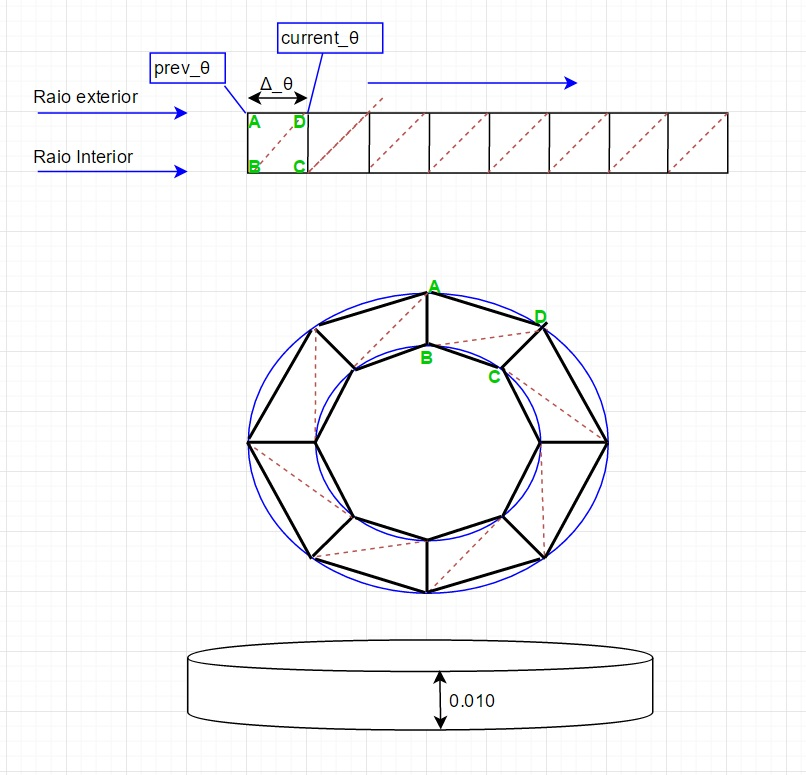
\includegraphics[width=\textwidth,height=\textheight,keepaspectratio]{resources/disco.jpg}
 	\captionsetup{type=figure, width=0.8\linewidth}
	\caption{Diagrama Disco}
\label{fig:ssec1:disc} 
\end{center}

Como se pode verificar o diagrama é relativamente semelhante ao da esfera.
A matriz aqui observada apenas tem uma linha porque não se consideram
\textit{stacks} na representação do disco. As 8 colunas que representam as
8 \textit{slices} (estas 8 slides servem meramente para propósitos
exemplificativos). 


\begin{center}
 	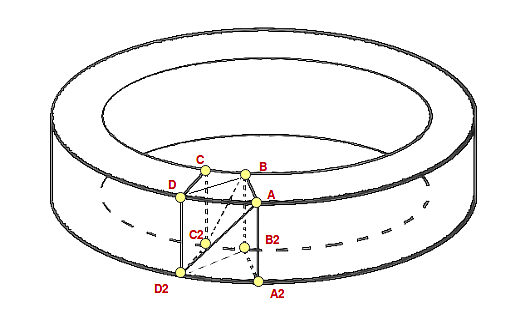
\includegraphics[width=\textwidth,height=0.5\textheight,keepaspectratio]{resources/discodiagram.png}
 	\captionsetup{type=figure, width=0.8\linewidth}
	\caption{Pormenor dos vértices para desenho de um disco}
\label{fig:sec1:disc:vertex} 
\end{center}

Como se pode observar, o raciocínio é desenhar quadricula a quadricula com dois
triângulos cada, neste exemplo verifica-se que a primeira quadricula
é constituída pelos triângulos ABD e BCD.\ As coordenadas de cada ponto (vértice
dos triângulos) são calculados com o auxílio das variáveis angulares
prev\_$\theta $ e current\_$\theta$ usando a formulação das coordenadas
esféricas. A diferença entre esta é o comprimento/largura da quadricula que
corresponde a $\dfrac{2\pi}{slices}$. 

Ora este processo é referente à face superior do disco. Para desenhar a face
inferior faz-se o mesmo processo mas com outros vértices equivalentes nos eixos
\emph{xx} e \emph{zz} mas com uma diferença fixa de 0.010 \emph{yy} para
representar a altura.

Quanto à face lateral do disco o processo é idêntico ao representado na matriz
acima, mas enquanto que, para representar tanto a face superior como a inferior,
os pontos usados têm todos os o mesmo valor \emph{yy}, para representar o lado do disco
usa-se uma combinação dos pontos de ambas as faces. 

Este processo está representado no \emph{Algoritmo~\ref{alg:sec1:disco}},
e um resultado figura na \emph{Figura~\ref{fig:sec1:disc:res1}} e na
\emph{Figura~\ref{fig:sec1:disc:res2}}.  

\begin{center}
 	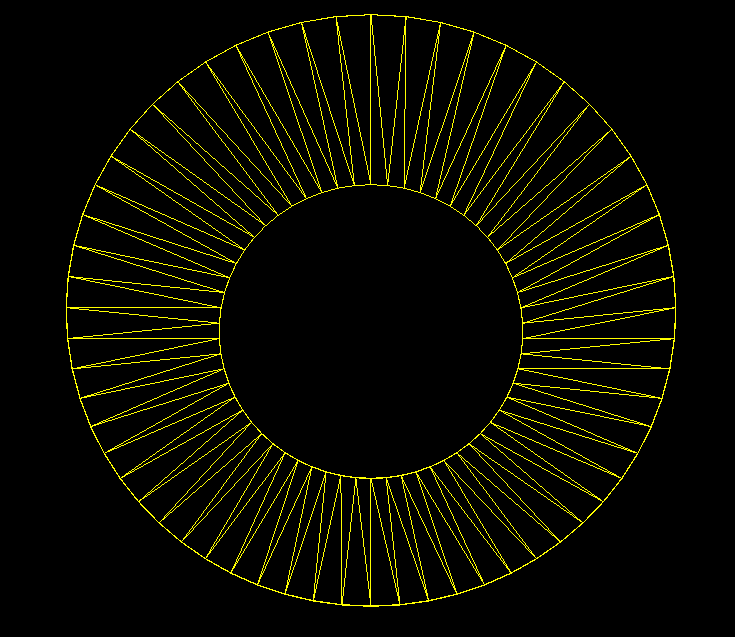
\includegraphics[width=\textwidth,height=0.5\textheight,keepaspectratio]{resources/disco1.png}
 	\captionsetup{type=figure, width=0.8\linewidth}
	\caption{Resultado de um disco em \emph{wireframe}, visto de baixo}
\label{fig:sec1:disc:res1} 
\end{center}


\begin{center}
 	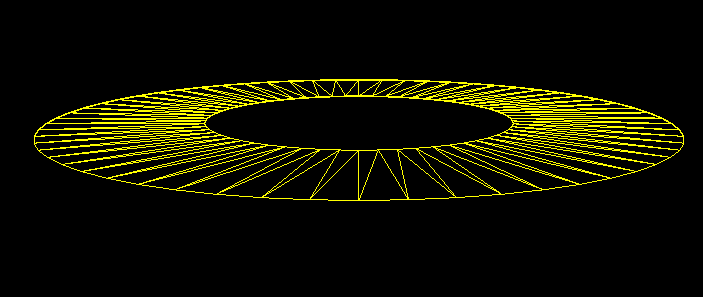
\includegraphics[width=\textwidth,height=0.5\textheight,keepaspectratio]{resources/disco2.png}
 	\captionsetup{type=figure, width=0.8\linewidth}
	\caption{Resultado de um disco em \emph{wireframe}, visto de outro ângulo}
\label{fig:sec1:disc:res2} 
\end{center}




\newgeometry{margin=1cm}
\begin{landscape}
\thispagestyle{empty} %% Remove header and footer.
\begin{algorithm}
\caption{Disco}\label{alg:sec1:disco}

\begin{center}
%\footnotesize %% Smaller font size.

\begin{algorithmic}[1]
\State$\Delta\_\theta \gets \dfrac{2\pi}{slices}$


\State$prev\_\theta \gets 0$
\State$current\_\theta \gets \Delta\_\theta$

\State$i \gets 0$


\While{$i \leq slices$} 

\State$Ponto A \gets raioOut*\sin(prev\_\theta),
 0.005,
 raioOut*\cos(prev\_\theta)$

\State$Ponto B \gets raioIn*\sin(prev\_\theta),
 0.005,
 raioIn*\cos(prev\_\theta)$

\State$Ponto C \gets raioIn*\sin(current\_\theta),
 0.005,
 raioIn*\cos(current\_\theta)$

\State$Ponto D \gets raioOut*\sin(current\_\theta),
  0.005,
 raioOut*\cos(current\_\theta)$

\State$Ponto A2 \gets raioOut*\sin(prev\_\theta),
 -0.005,
 raioOut*\cos(prev\_\theta)$

\State$Ponto B2 \gets raioIn*\sin(prev\_\theta),
 -0.005,
 raioIn*\cos(prev\_\theta)$

\State$Ponto C2 \gets raioIn*\sin(current\_\theta),
 -0.005,
 raioIn*\cos(current\_\theta)$

\State$Ponto D2 \gets raioOut*\sin(current\_\theta),
  -0.005,
 raioOut*\cos(current\_\theta)$




\Comment{Lado de cima}

\State$Triangulo(Ponto D, Ponto B, Ponto A)$ \Comment{Guardado em ficheiro}
\State$Triangulo(Ponto C, Ponto B, Ponto D)$ \Comment{Guardado em ficheiro}



\Comment{Lado de baixo}
\State$Triangulo(Ponto A2, Ponto B2, Ponto D2)$ \Comment{Guardado em ficheiro}
\State$Triangulo(Ponto D2, Ponto B2, Ponto C2)$   \Comment{Guardado em ficheiro}
		  
\Comment{Lado de externo}
\State$Triangulo(Ponto A2, Ponto A, Ponto D2)$\Comment{Guardado em
ficheiro}
\State$Triangulo(Ponto D, Ponto D2, Ponto A)$\Comment{Guardado em
ficheiro}
  
\Comment{Lado de interno}
\State$Triangulo(Ponto B, Ponto C2, Ponto B2)$\Comment{Guardado em
ficheiro}
\State$Triangulo(Ponto C, Ponto C2, Ponto B)$\Comment{Guardado em
ficheiro}



\State$prev\_\theta \gets current\_\theta$
\State$current\_\theta \gets current\_\theta + \Delta\_\theta$

\State$i \gets i + 1$


\EndWhile{}
\end{algorithmic}
\end{center}

\end{algorithm}


\end{landscape}
\restoregeometry{}
